\documentclass[aspectratio=169, table]{beamer}

\usepackage{colortbl}
\usepackage{xcolor}
\usepackage{listings}
\usepackage{tikz}
\usepackage{pgfplots}
\usepgfplotslibrary{polar}
\usetikzlibrary{arrows.meta, positioning, calc}

\usetheme{Pradita}



\lstdefinelanguage{bash} {
	keywords={},
	basicstyle=\ttfamily\small,
	keywordstyle=\color{blue}\bfseries,
	ndkeywords={iex},
	ndkeywordstyle=\color{purple}\bfseries,
	sensitive=true,
	commentstyle=\color{gray},
	stringstyle=\color{red},
	numbers=left,
	numberstyle=\tiny\color{gray},
	breaklines=true,
	frame=lines,
	backgroundcolor=\color{lightgray!10},
	tabsize=2,
	comment=[l]{\#},
	morecomment=[s]{/*}{*/},
	commentstyle=\color{gray}\ttfamily,
	stringstyle=\color{purple}\ttfamily,
	showstringspaces=false,
	captionpos=b
}

% Define Python language style for listings
\lstdefinestyle{PythonStyle}{
    language=Python,
    basicstyle=\ttfamily\footnotesize,
    keywordstyle=\color{blue}\bfseries,
    commentstyle=\color{gray}\itshape,
    stringstyle=\color{red},
    showstringspaces=false,
    breaklines=true,
    frame=lines,
    numbers=left,
    numberstyle=\tiny\color{gray},
    backgroundcolor=\color{lightgray!10},
    tabsize=4,
    captionpos=b
}


\title{\Huge Security in \\
	Software Systems\vspace{8pt}}
\subtitle{IT140704 - Big Data for Business}
%\date[Serial]{Penggunaan Large Language Model untuk Pengajaran}
\author{\textbf{Alfa Yohannis}}
\begin{document}
	
	\frame{\titlepage}
	

	\begin{frame}[fragile]
		\frametitle{Contents}
		\vspace{20pt}
		\begin{columns}[t]
			\column{0.5\textwidth}
			\tableofcontents[sections={1-5}]
			
			\column{0.5\textwidth}
			\tableofcontents[sections={6-20}]
		\end{columns}
	\end{frame}
	
	\begin{frame}{\hfill}
		\centering
		\Huge{\textbf{What can we do to secure our software systems?}}
	\end{frame}
	

\section{Pengantar Security}

	\begin{frame}{\hfill}
		\centering
		\Huge{\textbf{Pengantar Security}}
	\end{frame}

\begin{frame}{Keamanan Sistem Perangkat Lunak}
	\vspace{10pt}
	\begin{itemize}
		\item Pengembangan sistem modern menyatukan aktivitas perancangan, implementasi, dan pengelolaan sistem yang berjalan.
		\item Pendekatan ini menekankan kolaborasi, automasi, dan umpan balik cepat dari sistem yang sedang beroperasi.
		\item Dalam banyak praktik awal, \textbf{keamanan} sering diperlakukan sebagai aktivitas terpisah atau tahap tambahan di akhir.
		\item Pendekatan yang lebih matang menempatkan security sebagai bagian inheren dari seluruh siklus hidup sistem.
	\end{itemize}
	
	\vspace{6pt}
	{\footnotesize Fokus bergeser: dari keamanan sebagai aktivitas terpisah menjadi keamanan sebagai properti sistem}
\end{frame}


\begin{frame}{Security sebagai Kontrol Perilaku Sistem}
	\vspace{10pt}
	\begin{itemize}
		\item Sistem modern bersifat kompleks, terdistribusi, dan terus berubah, sehingga keamanan tidak dapat dipusatkan di satu tahap.
		\item Kesalahan desain, implementasi, dan operasi masing-masing menciptakan risiko keamanan yang berbeda.
		\item Security dipahami sebagai \textbf{kontrol terhadap perilaku sistem}, bukan sekadar keberadaan fitur atau mekanisme.
		\item Keamanan sistem bersifat \emph{akumulatif}: setiap kontrol hanya mengurangi sebagian risiko.
	\end{itemize}
	
	\vspace{6pt}
	{\footnotesize Fokus bab ini: bagaimana kontrol keamanan memengaruhi perilaku runtime sistem}
\end{frame}


\section{Tingkatan Security dalam Pengembangan Sistem}

	\begin{frame}{\hfill}
		\centering
		\Huge{\textbf{Tingkatan Security dalam Pengembangan Sistem}}
	\end{frame}

\begin{frame}{Tingkatan Security dalam Siklus Sistem}
	\vspace{10pt}
	\begin{itemize}
		\item Keamanan sistem tidak hadir sebagai satu mekanisme tunggal, melainkan sebagai \textbf{lapisan kontrol} di berbagai tahap siklus hidup.
		\item Setiap tahap memiliki karakteristik risiko dan jenis ancaman yang berbeda.
		\item Konsekuensinya, keamanan sistem bersifat \textbf{kumulatif}:
		      setiap tahap hanya mengurangi \emph{sebagian} risiko.
		\item Kontrol pada tahap akhir tidak dapat sepenuhnya menambal keputusan yang salah pada tahap awal.
		\item \textbf{Contoh:}
		      \textbf{(1)} Desain tanpa \emph{pembatasan hak akses}
		      $\rightarrow$ enkripsi runtime tetap membiarkan data sensitif tersebar ke komponen yang tidak perlu.
		      \textbf{(2)} Kode tanpa \emph{validasi input}
		      $\rightarrow$ firewall atau TLS tidak mencegah manipulasi data berbahaya.
	\end{itemize}
	
	\vspace{4pt}
	{\footnotesize Intuisi: keamanan adalah akumulasi keputusan kecil yang konsisten, bukan satu ``tes akhir''}
\end{frame}



\begin{frame}{Security pada Tahap Desain dan Implementasi}
	\vspace{10pt}
	\begin{columns}[t]
		\column{0.5\textwidth}
		\textbf{1. Tahap Desain}
		\begin{itemize}
			\item Membatasi sistem secara konseptual sebelum kode ditulis.
			\item \emph{Threat modeling}: identifikasi aset, alur data kritis, dan potensi ancaman.
			\item \emph{Trust boundary}: memisahkan komponen dipercaya vs tidak dipercaya.
			\item Output: keputusan arsitektur dan kebutuhan kontrol tahap berikutnya.
		\end{itemize}
		
		\column{0.5\textwidth}
		\textbf{2. Tahap Implementasi}
		\begin{itemize}
			\item Mencegah celah teknis pada level kode dan struktur program.
			\item Validasi + sanitasi input dari luar sistem.
			\item Gunakan library/framework yang teruji untuk crypto dan networking.
			\item Output: kode yang meminimalkan bug yang dapat dieksploitasi.
		\end{itemize}
	\end{columns}
	
	\vspace{6pt}
	{\footnotesize Desain membatasi ruang risiko; implementasi mencegah celah teknis yang langsung dieksploitasi}
\end{frame}


\begin{frame}{Tahap Build, Deployment, \& Runtime}
	\vspace{10pt}
	\begin{columns}[T]
		\column{0.3\textwidth}
		\textbf{3. Build \& Artifact}
		\begin{itemize}
			\item Risiko tersembunyi dari pihak ketiga.
			\item Pemeriksaan dependensi (kerentanan yang diketahui).
			\item \emph{Image hardening}: hilangkan komponen tidak perlu.
		\end{itemize}
		
		\column{0.37\textwidth}
		\textbf{4. Deployment \& Environment}
		\begin{itemize}
			\item Konfigurasi salah dapat membatalkan kontrol sebelumnya.
			\item \emph{Least privilege} untuk setiap service.
			\item Rahasia tidak ditanam di kode; dikelola via konfigurasi runtime/secret manager.
		\end{itemize}
		
		\column{0.34\textwidth}
		\textbf{5. Runtime \& Eksekusi}
		\begin{itemize}
			\item Sistem bertemu kondisi nyata yang tidak sepenuhnya terprediksi.
			\item Enkripsi payload antar komponen.
			\item Pembatasan aksi komponen saat berjalan (mis. read-only).
		\end{itemize}
	\end{columns}
	
	\vspace{12pt}
	{\footnotesize Pertemuan kali ini menekankan \textbf{runtime control}: bagaimana kontrol mengubah perilaku sistem yang sedang berjalan}
\end{frame}

\section{Penekanan Keamanan pada Pertemuan Kali Ini}
	\begin{frame}{\hfill}
		\centering
		\Huge{\textbf{Penekanan Keamanan pada Pertemuan Kali Ini}}
	\end{frame}

\begin{frame}{Posisi Sesi Ini dalam Lapisan Keamanan}
	\vspace{10pt}
	\begin{itemize}
		\item Pertemuan kali ini \textbf{tidak} membahas seluruh spektrum keamanan,
		      seperti analisis kerentanan statis, pengujian penetrasi,
		      manajemen identitas dan akses, maupun keamanan jaringan tingkat rendah.
		\item Fokus pertemuan kali ini adalah \textbf{keamanan runtime}:
		      kontrol yang aktif saat sistem berjalan dan berinteraksi dengan lingkungan operasional nyata.
		\item Contoh yang digunakan, yaitu enkripsi payload,
		      menunjukkan bagaimana satu kontrol runtime mengubah perilaku sistem,
		      sekaligus menegaskan keterbatasannya.
	\end{itemize}
\end{frame}

\section{Arsitektur Sistem Studi Kasus}

	\begin{frame}{\hfill}
		\centering
		\Huge{\textbf{Arsitektur Sistem Studi Kasus}}
	\end{frame}

\begin{frame}{Arsitektur Sistem dengan Enkripsi Payload}
	\vspace{14pt}
	\centering
	\scalebox{0.8}{
	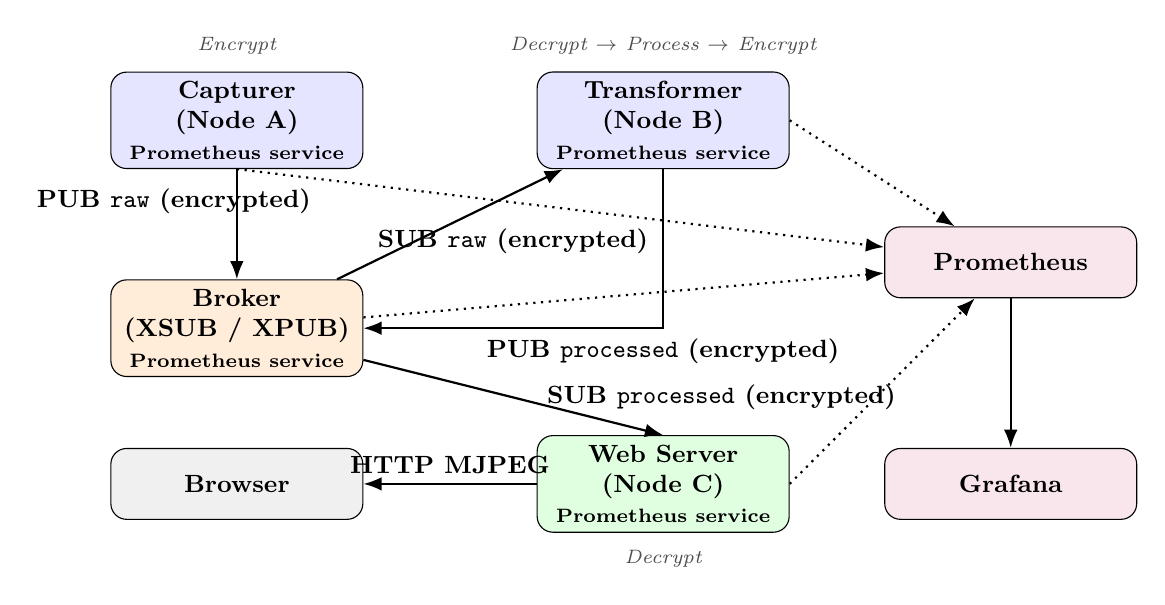
\begin{tikzpicture}[
	  font=\small\bfseries,
	  node distance=9mm and 12mm,
	  box/.style={
	    draw,
	    rounded corners=2mm,
	    align=center,
	    minimum width=32mm,
	    minimum height=9mm,
	    fill=blue!10
	  },
	  brokerbox/.style={box,fill=orange!15},
	  webbox/.style={box,fill=green!12},
	  browserbox/.style={box,fill=gray!12},
	  extbox/.style={box,fill=purple!10},
	  annot/.style={font=\scriptsize\itshape, text=black!70},
	  arrow/.style={-Latex,thick},
	  dottedarrow/.style={-Latex,thick,dotted}
	]
	
	% Core nodes
	\node[box] (transformer) {Transformer\\(Node B)\\{\scriptsize Prometheus service}};
	\node[annot, above=1mm of transformer] {Decrypt $\rightarrow$ Process $\rightarrow$ Encrypt};
	
	\node[box,left=of transformer, xshift=-10mm] (capturer) {Capturer\\(Node A)\\{\scriptsize Prometheus service}};
	\node[annot, above=1mm of capturer] {Encrypt};
	
	\node[brokerbox, below=of capturer, yshift=-5mm] (broker) {Broker\\(XSUB / XPUB)\\{\scriptsize Prometheus service}};
	
	\node[browserbox,below=of broker] (browser) {Browser};
	
	\node[webbox,right=of browser, xshift=10mm](web) {Web Server\\(Node C)\\{\scriptsize Prometheus service}};
	\node[annot, below=1mm of web] {Decrypt};
	
	% External observability nodes
	\node[extbox,right=of web] (grafana) {Grafana};
	\node[extbox,above=of grafana, yshift=10mm] (prom) {Prometheus};
	
	% Data flow arrows (encrypted payload)
	\draw[arrow] (capturer) -- 
	  node[above, xshift=-8mm]{PUB \texttt{raw} (encrypted)} 
	  (broker);
	
	\draw[arrow] (broker) -- 
	  node[above, yshift=-5mm, xshift=8mm]{SUB \texttt{raw} (encrypted)} 
	  (transformer);
	
	\draw[arrow] (transformer.south) |- 
	  node[below]{PUB \texttt{processed} (encrypted)} 
	  (broker.east);
	
	\draw[arrow] (broker) -- 
	  node[right,xshift=3mm]{SUB \texttt{processed} (encrypted)} 
	  (web.north);
	
	\draw[arrow] (web.west) -- 
	  node[above]{HTTP MJPEG} 
	  (browser.east);
	
	% Observability
	\draw[dottedarrow] (capturer.south) -- (prom);
	\draw[dottedarrow] (broker) -- (prom);
	\draw[dottedarrow] (transformer.east) -- (prom);
	\draw[dottedarrow] (web.east) -- (prom);
	\draw[arrow] (prom) -- (grafana);
	
	\end{tikzpicture}
	}

	{\footnotesize Enkripsi dan dekripsi dilakukan pada node produsen dan konsumen; broker meneruskan pesan tanpa akses ke isi payload}
\end{frame}


\begin{frame}{Arsitektur Sistem Studi Kasus}
	\vspace{10pt}
	\begin{itemize}
		\item Sistem menggunakan pola komunikasi \emph{publish--subscribe} dengan broker sebagai perantara pertukaran pesan.
		\item Produsen dan konsumen data tidak saling mengenal secara langsung, sehingga sistem bersifat terbuka dan berikatan longgar.
		\item Broker berperan netral: meneruskan pesan berdasarkan topik tanpa memahami atau memodifikasi isi payload.
		\item Risiko utama muncul pada observasi lalu lintas pesan, karena broker dan jaringan dapat diakses oleh pihak luar.
		\item Kontrol keamanan diterapkan pada saat sistem berjalan melalui \textbf{enkripsi payload} di sisi penghasil dan pemroses data.
		\item Sepanjang jalur komunikasi melalui broker, payload selalu berada dalam keadaan terenkripsi.
	\end{itemize}
\end{frame}

\section{Eksperimen dan Validasi Kontrol Keamanan Runtime}

	\begin{frame}{\hfill}
		\centering
		\Huge{\textbf{Eksperimen dan Validasi Kontrol Keamanan Runtime}}
	\end{frame}

\begin{frame}{\LARGE{Langkah\textsuperscript{2} Eksperimen Kontrol Keamanan Runtime}}
	\vspace{10pt}
	\begin{enumerate}
		\item \textbf{Menjalankan sistem tanpa kontrol keamanan},
		      sehingga payload yang melewati broker dapat diamati dan dibaca sebagai data mentah.
		\item \textbf{Menambahkan kontrol enkripsi payload}
		      tanpa mengubah arsitektur dasar sistem, dengan mengenkripsi data sebelum publikasi dan mendekripsi setelah konsumsi.
		\item \textbf{Menjalankan kembali sistem}
		      dengan konfigurasi yang sama, kecuali penambahan kunci enkripsi sebagai kebijakan runtime.
		\item \textbf{Melakukan observasi lalu lintas pesan}
		      pada sisi broker atau jaringan oleh pihak yang tidak memiliki kunci enkripsi.
		\item \textbf{Membandingkan hasil observasi}
		      sebelum dan sesudah enkripsi, khususnya perbedaan antara data yang terlihat dan data yang dapat dibaca.
	\end{enumerate}
	
	\vspace{6pt}
	{\footnotesize Validasi dilakukan melalui perubahan perilaku sistem yang dapat diamati secara empiris}
\end{frame}

\subsection*{Generasi Kunci Enkripsi sebagai Kebijakan Runtime}

\begin{frame}[fragile]{Generasi Kunci Enkripsi Payload}
	\vspace{6pt}
	\begin{columns}[t]
		\column{0.6\textwidth}
		\begin{lstlisting}[style=PythonStyle, caption={Generate Fernet key for payload encryption}]
from cryptography.fernet import Fernet

# generate symmetric encryption key
key = Fernet.generate_key()

# print as Base64 string
print(key.decode())
		\end{lstlisting}
		
		\column{0.4\textwidth}
		\begin{itemize}
			\item Kunci dihasilkan satu kali sebelum sistem dijalankan.
			\item Digunakan sebagai kebijakan keamanan runtime.
			\item Didistribusikan melalui konfigurasi lingkungan.
			\item Tidak tertanam di dalam kode aplikasi.
		\end{itemize}
	\end{columns}
	
	\vspace{6pt}
	{\footnotesize Kunci enkripsi diperlakukan sebagai artefak kebijakan operasional, terpisah dari logika aplikasi}
\end{frame}

\subsection*{Konfigurasi Kunci pada \texttt{docker-compose.yml}}

\begin{frame}[fragile]{Konfigurasi Kunci Enkripsi pada Layanan}
	\vspace{20pt}
	\begin{columns}[T]
		\column{0.5\textwidth}
		\begin{lstlisting}[language=bash, basicstyle=\ttfamily\tiny, caption={Inject PAYLOAD\_KEY via docker-compose environment}]
services:
  transformer:
	...
    environment:
      - PAYLOAD_KEY=put the generated key here
  ...  
  capturer:
    ...
    environment:
      - PAYLOAD_KEY=put the generated key here
  ...
  web:
    ...
    environment:
      - PAYLOAD_KEY=put the generated key here
  ...
  broker:
    ...
    # intentionally no PAYLOAD_KEY here
\end{lstlisting}
		
		\column{0.5\textwidth}
		\begin{itemize}
			\item Kunci diberikan hanya pada komponen yang memproduksi atau mengonsumsi payload.
			\item Broker tidak menerima kunci enkripsi.
			\item Kebijakan keamanan diwujudkan melalui konfigurasi runtime.
			\item Tidak ada perubahan pada kode aplikasi.
		\end{itemize}

		\vspace{4pt}
	{\footnotesize Pembatasan akses data dicapai melalui distribusi kunci, bukan melalui kepercayaan pada komponen perantara}
	\end{columns}
\end{frame}

\subsection*{Dependensi Python pada Dockerfile}

\begin{frame}[fragile]{Dependensi Runtime pada Dockerfile}
	\vspace{6pt}
	\begin{columns}[t]
		\column{0.6\textwidth}
		\begin{lstlisting}[language=bash, caption={Install Python deps including encryption support}]
...
# ---- python deps (capturer / transformer runtime)
RUN pip install --no-cache-dir \
    pyzmq \
    opencv-python-headless \
    prometheus-client \
    psutil \
    cryptography
...
		\end{lstlisting}
		
		\column{0.4\textwidth}
		\begin{itemize}
			\item Dependensi ditetapkan pada tahap build.
			\item Enkripsi diperlakukan setara dengan pipeline data.
			\item Digunakan bersama komunikasi, observabilitas, dan pemrosesan.
			\item Tidak ditambahkan secara ad-hoc di runtime.
		\end{itemize}
	\end{columns}
	
	\vspace{4pt}
	{\footnotesize Enkripsi diposisikan sebagai bagian integral dari runtime pipeline, bukan fitur tambahan}
\end{frame}

\subsection*{Fungsi Enkripsi dan Dekripsi (Shared Library)}

\begin{frame}[fragile]{Fungsi Enkripsi dan Dekripsi Payload}
	\vspace{6pt}
	\begin{columns}[t]
		\column{0.7\textwidth}
		\begin{lstlisting}[style=PythonStyle, caption={Shared crypto helpers using PAYLOAD\_KEY }]
import os
from cryptography.fernet import Fernet

_PAYLOAD_KEY = os.environ["PAYLOAD_KEY"].encode()
_cipher = Fernet(_PAYLOAD_KEY)

def encrypt_bytes(data: bytes) -> bytes:
    return _cipher.encrypt(data)

def decrypt_bytes(token: bytes) -> bytes:
    return _cipher.decrypt(token)
		\end{lstlisting}
		
		\column{0.3\textwidth}
		\begin{itemize}
			\item Modul bersama untuk semua layanan.
			\item Kunci dibaca dari konfigurasi runtime.
			\item Tidak ada kunci tertanam di kode.
			\item Fungsi simetris untuk payload biner.
		\end{itemize}
	\end{columns}
	
	\vspace{4pt}
	{\footnotesize Kontrol enkripsi direalisasikan sebagai fungsi runtime yang konsisten lintas komponen}
\end{frame}

\subsection*{Integrasi pada Transformer: Decrypt--Process--Encrypt}

\begin{frame}[fragile]{Integrasi Enkripsi pada Node Transformer}
	\vspace{6pt}
	\begin{columns}[t]
		\column{0.7\textwidth}
		\begin{lstlisting}[style=PythonStyle, basicstyle=\ttfamily\scriptsize, caption={Transformer decrypts input and encrypts output payload}]
# receive encrypted parts from broker
enc_header_b, enc_jpeg_in = recv_parts()

# decrypt at runtime
header_b = decrypt_bytes(enc_header_b)
jpeg_in  = decrypt_bytes(enc_jpeg_in)

# process (decode -> transform -> encode)
out_header_b, jpeg_out = process_frame(header_b, jpeg_in)

# encrypt again before publishing
enc_out_header = encrypt_bytes(out_header_b)
enc_jpeg_out   = encrypt_bytes(jpeg_out)

send_parts(enc_out_header, enc_jpeg_out)
		\end{lstlisting}
		
		\column{0.3\textwidth}
		\begin{itemize}
			\item Dekripsi hanya pada node berwenang.
			\item Pemrosesan terjadi pada data asli.
			\item Enkripsi ulang sebelum publikasi.
			\item Perilaku runtime berubah tanpa ubah arsitektur.
		\end{itemize}
			\vspace{4pt}
	{\footnotesize Kontrol keamanan bekerja pada alur eksekusi nyata: decrypt--process--encrypt}
	\end{columns}
\end{frame}

\subsection*{Kode Uji Lokal: Validasi Enkripsi dan Kunci}

\begin{frame}[fragile]{Uji Lokal Enkripsi dan Validasi Kunci}
	\vspace{6pt}
	\begin{columns}[t]
		\column{0.6\textwidth}
		\begin{lstlisting}[style=PythonStyle,basicstyle=\ttfamily\tiny, caption={Quick test: encrypt/decrypt roundtrip}]
import os
from cryptography.fernet import Fernet, InvalidToken

key = os.environ["PAYLOAD_KEY"].encode()
cipher = Fernet(key)

plain = b"header:frame=1;ts=123456"
token = cipher.encrypt(plain)

assert token != plain
assert cipher.decrypt(token) == plain

try:
    wrong = Fernet(Fernet.generate_key())
    wrong.decrypt(token)
    raise AssertionError("Should not decrypt with wrong key")
except InvalidToken:
    pass

print("OK: encryption on, wrong key fails, correct key succeeds.")
		\end{lstlisting}
		
		\column{0.4\textwidth}
		\begin{itemize}
			\item Payload terenkripsi berbeda dari data asli.
			\item Dekripsi berhasil hanya dengan kunci benar.
			\item Kunci salah menghasilkan kegagalan.
			\item Konsep: data terlihat tetapi tidak terbaca.
		\end{itemize}

			\vspace{4pt}
	{\footnotesize Uji minimum untuk memverifikasi kontrol enkripsi sebelum eksperimen runtime}
	\end{columns}
	

\end{frame}

\subsection*{Validasi Observasional: Sniffer sebagai Representasi Ancaman}

\begin{frame}[fragile]{Validasi Observasional dengan Sniffer}
	\vspace{6pt}
	\begin{columns}[t]
		\column{0.7\textwidth}
		\begin{lstlisting}[style=PythonStyle, basicstyle=\ttfamily\scriptsize, caption={Sniffer view: visible bytes, unreadable without key}]
def hexdump(b: bytes, n: int = 32) -> str:
    return b[:n].hex()

# captured payload (e.g., from network observation)
captured = token  # placeholder for wire-captured bytes
print("Visible (first bytes):", hexdump(captured))

# no key available -> decryption must fail
from cryptography.fernet import Fernet, InvalidToken
try:
    Fernet(Fernet.generate_key()).decrypt(captured)
except InvalidToken:
    print("Unreadable: decrypt failed without the correct key.")
		\end{lstlisting}
		
		\column{0.3\textwidth}
		\begin{itemize}
			\item Observasi pasif tanpa kunci enkripsi.
			\item Payload tetap terlihat di jaringan.
			\item Isi data tidak dapat ditafsirkan.
			\item Bukti perubahan perilaku runtime.
		\end{itemize}
		
		{\footnotesize Data dapat diamati, tetapi keterbacaan dibatasi oleh kebijakan kunci pada runtime}
	\end{columns}
	
\end{frame}

\subsection*{Validasi Observasional: Perbandingan Output Sniffer}

\begin{frame}[fragile]{Output Sniffer: Sebelum vs Sesudah Enkripsi}
	\vspace{6pt}
	\begin{columns}[t]
		\column{0.5\textwidth}
		\textbf{Tanpa Enkripsi}
		\begin{lstlisting}[style=PythonStyle, basicstyle=\ttfamily\scriptsize]
Visible (first bytes):
ffd8ffe000104a464946000101...
Readable:
JPEG header detected
		\end{lstlisting}
		\begin{itemize}
			\item Byte awal \texttt{FF D8 FF}
			\item Dikenal sebagai \emph{JPEG signature}
			\item Format file dapat ditebak
			\item Isi payload bermakna
		\end{itemize}
		
		\column{0.5\textwidth}
		\textbf{Dengan Enkripsi Payload}
		\begin{lstlisting}[style=PythonStyle, basicstyle=\ttfamily\scriptsize]
Visible (first bytes):
674141414141426d4e6d6c5a...
Unreadable:
decrypt failed without key
		\end{lstlisting}
		\begin{itemize}
			\item Tidak ada pola tetap
			\item Signature format hilang
			\item Byte tampak acak
			\item Isi payload tidak dapat dibaca
		\end{itemize}
	\end{columns}
	
	\vspace{10pt}
	{\footnotesize JPEG dapat dikenali melalui \emph{magic bytes} \texttt{FF D8 FF}; enkripsi menghilangkan pola ini}
\end{frame}



\section{Diskusi dan Refleksi}
	\begin{frame}{\hfill}
		\centering
		\Huge{\textbf{Diskusi dan Refleksi}}
	\end{frame}

\begin{frame}{Pertanyaan Refleksi}
	\vspace{10pt}
	\begin{enumerate}
		\item Apa risiko yang muncul ketika sistem berjalan tanpa kontrol keamanan runtime,
		      meskipun sistem terlihat berfungsi normal?
		\item Bagaimana satu kontrol sederhana, seperti enkripsi payload,
		      dapat mengubah perilaku sistem tanpa mengubah arsitekturnya?
		\item Mengapa satu kontrol keamanan tidak cukup untuk menyebut suatu sistem aman?
		\item Kontrol keamanan tambahan apa yang perlu dipertimbangkan
		      pada tahap lain selain runtime?
		\item Apakah kontribusi observabilitas terhadap keamanan sistem?
	\end{enumerate}
	
	\vspace{6pt}
	{\footnotesize Pertanyaan ditujukan untuk mendorong refleksi lintas peran dan tingkat teknis}
\end{frame}


\section{Rangkuman}

	\begin{frame}{\hfill}
		\centering
		\Huge{\textbf{Rangkuman}}
	\end{frame}

\begin{frame}{Rangkuman}
	\vspace{10pt}
	\begin{itemize}
		\item Keamanan sistem bersifat berlapis dan tidak dapat dipusatkan pada satu mekanisme.
		\item Keamanan dipahami sebagai kontrol terhadap perilaku sistem yang sedang berjalan.
		\item Studi kasus menunjukkan bahwa enkripsi payload membatasi keterbacaan data
		      tanpa mengubah alur atau arsitektur sistem.
		\item Kunci enkripsi berperan sebagai kebijakan runtime yang dikelola secara operasional.
		\item Observabilitas memungkinkan efektivitas kontrol keamanan diuji dan divalidasi secara empiris.
	\end{itemize}
	
	\vspace{6pt}
	{\footnotesize Keamanan yang baik adalah keamanan yang dapat diamati dan dibuktikan}
\end{frame}

\end{document}
